\vspace{0.5mm}\hrule\vspace{0.5mm}
\section{Tabular Reinforcement Learning}

% Trajectory $\tau$: \scalebox{0.9}{$\tau \defeq (\tau_0, \tau_1, \dots)$}, with \scalebox{0.9}{$\tau_i \defeq (x_i, a_i, r_i, x_{i+1})$}.

% \begin{itemize}
%     \item \textbf{On-policy}: Agent can choose any policy.
%     \item \textbf{Off-policy}: No choice of policy.
%     \item \textbf{Model-based} Learn the underlying MDP.
%     \item \textbf{Model-free} Learn the value function directly.
% \end{itemize}

Markovian property of the underlying MDP: \scalebox{0.8}{$X_{t=1} \bot X_{t'+1} \mid X_t, X_{t'+1},A_t,A_{t'}$}\hfill \scalebox{0.8}{$R_t \bot X_{t'} \mid R_t, X_{t'+1},A_t,A_{t'}$}

\begin{framed}
    \textbf{Bootstrapping:} approx. a true quantity by using an empirical quantity, which itself is constructed using samples from the true quantity that is to be approx. 
\end{framed}

\begin{framed}
    \textbf{For model-based approaches MLE yields:}\\
    \scalebox{0.8}{${\hat{p}(x' \mid x, a) = \frac{N(x' \mid x, a)}{N(a \mid x)}}$} and \scalebox{0.8}{${\hat{r}(x, a) = \frac{1}{N(a \mid x)} \sum_{t = 0, x_t = x,a_t = a}^\infty r_t}$}
    Both unbiased as they correspond to a sample mean.
    \begin{itemize}
        \item $N(x' \mid x, a)$ num. trans. from $x$ to $x'$ when play $a$
        \item $N(a \mid x)$ nums trans. from $x$ and play $a$.
    \end{itemize}
\end{framed}

\begin{framed}
    \textbf{Greedy in the limit with inf. exploration (GLIE)}:
    \begin{enumerate}
        \item All state-action pairs are explored infinitely many times: $\lim_{t \rightarrow \infty} N_t(x, a) = \infty$
        \item The policy converges to a greedy policy:\\[-0.5ex]
        $\lim_{t \rightarrow \infty} \pi_t(a \mid x) = \mathbf 1\{a = \argmax_{a' \in A} Q_t^\star(x, a')\}$
    \end{enumerate}
\end{framed}

\begin{framed}
    \textbf{Robbins-Montro (RM) conditions}: for a sequence\\[-0.5ex]
    $(\alpha)_{t \in \mathbb N_0}$ if: $\alpha_t \geq 0$, $\sum_{t=0}^{\infty}{\alpha_t} = \infty$, $\sum_{t=0}^{\infty}{\alpha_t^2} < \infty$.
\end{framed}

\vspace{0.5mm}\hrule\vspace{0.5mm}

\includegraphics[width=0.95\linewidth,trim={0 0.5cm 0 0.7cm},clip]{images/epsilon_greedy.png}

\begin{itemize}
    \item Ignores all past experience. \scalebox{0.7}{\textbullet} Will eventually converge.
    \item $\epsilon$-greedy is GLIE with prob. 1 if $(\epsilon_t)_{t \in \mathbb N_0}$ satisfies the\\[-0.5ex]
    \textbf{Robbins-Montro (RM)} conditions (e.g., $\epsilon_t = \sfrac1t$).
\end{itemize}

\vspace{0.5mm}\hrule\vspace{0.5mm}

\textbf{Softmax/Boltzmann exploration:} alt. to $\epsilon$-greedy $\pi_\lambda(a \mid x) \propto \exp(\frac1\lambda Q^\star(x, a))$ (Gibbs). For $\lambda \rightarrow 0$ greedily max. Q-fn. For $\lambda \rightarrow \infty$ uniform random exploration.

\vspace{0.5mm}\hrule\vspace{0.5mm}

\includegraphics[width=0.92\linewidth,trim={0 0.6cm 0 0.7cm},clip]{images/R_max.png}
\begin{tikzpicture}[baseline, overlay]
  \node[anchor=west, font=\fontsize{6pt}{6pt}\selectfont, anchor=base, xshift=-0.75cm, yshift=1.9cm, fill=yellow!10] at (0, 0) {
    On-policy, Model-based
  };
\end{tikzpicture}

\begin{itemize}
    \item Optimism in the face of uncertainty. Init. with max rew.
    \item Every $T$ steps, with high prob., either obtains near-\\optimal reward; or visits one unknown state-action pair.
    \item With prob. at least $1-\delta$, $R_\mathrm{max}$ reaches $\epsilon$-optimal $\pi$ in poly. num. steps in $\card{\sX}$, $\card{\sA}$, $T$, $\nicefrac{1}{\epsilon}$, $\nicefrac{1}{\delta}$, and $R_\mathrm{max}$.
\end{itemize}

\vspace{0.5mm}\hrule\vspace{0.5mm}

\includegraphics[width=0.85\linewidth,trim={0 1.2cm 0 0.8cm},clip]{images/TD_learning.png}
\begin{tikzpicture}[baseline, overlay]
  \node[anchor=west, font=\fontsize{6pt}{6pt}\selectfont, anchor=base, xshift=-0.6cm, yshift=0.8cm, fill=yellow!10] at (0, 0) {
    On-policy, Model-free
  };
\end{tikzpicture}

\begin{itemize}
    \item If $\alpha_t$ satisfies RM conditions and all state-action pairs are chosen inf. often, then $V^\pi$ conv. to $v^\pi$ w. prob 1.
    \item For estimates $V^\pi$ to converge true $v^\pi$, the transitions that are used for the estimation must follow policy $\pi$.
\end{itemize}

\vspace{0.5mm}\hrule\vspace{0.5mm}

\textbf{SARSA:} Same as TD but estimate $Q$ with update: $Q^\pi(x, a) \leftarrow (1-\alpha_t) Q^\pi(x, a) + \alpha_t (r + \gamma Q^\pi(x', a'))$
Same convergence guarantees as TD.
\begin{tikzpicture}[baseline, overlay]
  \node[anchor=west, font=\fontsize{6pt}{6pt}\selectfont, anchor=base, xshift=1cm, yshift=-0cm, fill=yellow!10] at (0, 0) {
    On-policy, Model-free
  };
\end{tikzpicture}

\vspace{0.5mm}\hrule\vspace{0.5mm}
\includegraphics[width=0.95\linewidth,trim={0 2cm 0 0.8cm},clip]{images/Q_learning.png}
\begin{tikzpicture}[baseline, overlay]
  \node[anchor=west, font=\fontsize{6pt}{6pt}\selectfont, anchor=base, xshift=-0.9cm, yshift=0.6cm, fill=yellow!10] at (0, 0) {
    Off-policy, Model-free
  };
\end{tikzpicture}

\begin{itemize}
    \item If $\alpha_t$ satisfies RM conditions and all state-action pair are visited inf. often, then $Q^\star$ conv. to $q^\star$ with prob. 1.
    \item With prob. at least $1 - \delta$, conv. to $\epsilon$-optimal policy in num. steps that is poly. in $\log |X|$, $\log |A|$, $\frac 1 \epsilon$ and $\log \frac1\delta$.
\end{itemize}

\vspace{0.5mm}\hrule\vspace{0.5mm}

\textbf{Optimistic Q-learning: Similar to $R_\text{max}$ Init.} \scalebox{0.8}{$Q^\star(x, a) = V_\text{max} \prod_{t=1}^{T_\text{init}} (1 - \alpha_t)^{-1}$} w. \scalebox{0.8}{$V_\text{max} \defeq \frac{R_\text{max}}{1 - \gamma} \ge \max q^\star(x, a)$}.

\begin{itemize}
    \item With prob. at least $1 - \delta$, $\epsilon$-optimal $\pi$ after num. steps that is poly. in $|X|$, $|A|$, $\frac1\epsilon$, $\log \frac1\delta$, and $R_\text{max}$ where init. time $T_\text{init}$ is upper bounded by a poly. in same coeff.
    \item If $T_\text{init}$ chosen large enough, converges quickly to $\pi^\star$.
\end{itemize}
